% IEEE PacificVis 2027 -- Conference Paper Track. VGTC conference template (2024.02.14).
% Restructured manuscript (2026-10-27, outline in OUTLINE.md). Figures and tables: scripts/make_figures.py.
% Compile: pdfLaTeX + BibTeX (Overleaf), or `tectonic -X compile main.tex`. Supplement: supplement.tex.
% Wide figures are defined one section before they are discussed so that they float into place.

\documentclass[review]{vgtc}                 % review version (double blind)
%\documentclass{vgtc}                         % final (conference style)

\usepackage{iftex}
\usepackage{graphicx}
\ifPDFTeX
  \pdfoutput=1\relax
  \pdfcompresslevel=9
  \pdfoptionpdfminorversion=7
\fi%
\DeclareGraphicsExtensions{.pdf,.png,.jpg,.jpeg}
\usepackage[T1]{fontenc}
\usepackage{mathptmx}
\renewcommand*\ttdefault{txtt}
\usepackage{booktabs}
\usepackage{cite}
\usepackage{amsmath,amssymb,amsthm}
\usepackage[noend]{algpseudocode}
\usepackage{algorithm}
\newtheorem{lemma}{Lemma}
\newtheorem{theorem}{Theorem}
\newtheorem{corollary}[theorem]{Corollary}
\newtheorem{definition}{Definition}
\newcommand{\dtop}{d_{\mathrm{top}}}
\newcommand{\lca}{\operatorname{lca}}
\newcommand{\nroe}{\mathrm{NROE}}
\newcommand{\pending}[1]{{\color{orange!80!black}[#1]}}
\newcommand{\takeaway}[1]{\noindent\emph{#1}\par\smallskip}
\setcounter{dbltopnumber}{2}\renewcommand{\dbltopfraction}{0.9}\renewcommand{\topfraction}{0.9}
\renewcommand{\bottomfraction}{0.8}\renewcommand{\textfraction}{0.07}\renewcommand{\floatpagefraction}{0.85}\renewcommand{\dblfloatpagefraction}{0.85}
\setlength{\textfloatsep}{9pt plus 2pt minus 2pt}
\setlength{\dbltextfloatsep}{9pt plus 2pt minus 2pt}

\title{Position-Faithful Merge Tree Maps:\\Certified Bounds and Optimal Layouts}
\author{Anonymous Authors}\onlineid{0}\vgtccategory{Research}\vgtcinsertpkg
\hypersetup{pdftitle={Position-Faithful Merge Tree Maps: Certified Bounds and Optimal Layouts}}

\abstract{Merge tree maps summarize a time-varying scalar field in one image: every time step becomes a one-dimensional profile whose basins are the features of the field, stacked along time. Existing maps keep the merge hierarchy and temporal coherence, but the axis then carries little spatial meaning, so a storm in the west may be drawn east of one in the east. We ask how close such a map can stay to a fixed spatial reference, such as longitude, without misrepresenting the hierarchy. We prove a closed-form lower bound on the order error of every map that preserves the merge tree, which holds for every method including TMTM and ST-MTM, a width-aware bound on the worst displacement for maps that place features as intervals, as ST-MTM and our method do, and chain-aware bounds for maps whose merge levels may err by a declared budget $\varepsilon$. We give layouts that attain them: a midpoint ordering, a width-aware search, and a budgeted ordering whose exact merge-level error is checked, combined with optimal barriers and a capped quadratic placement. The bounds do not depend on the dimension of the domain. A cross-method comparison on 917 frames from five planar and two volumetric sequences shows that most of the order error of existing maps is avoidable, that sorting by reference alone changes merge levels by up to 59\% of the scalar range, and that our exact maps lower the motion error of both previous methods on every sequence, while ST-MTM keeps the better distance preservation. Each of our maps reports two certified numbers, how far it moves features and how far it changes the hierarchy, and marks every changed merge on the map.}

\keywords{Merge trees, temporal scalar fields, topology-based visualization, one-dimensional layout, lower bounds.}

\teaser{
\centering
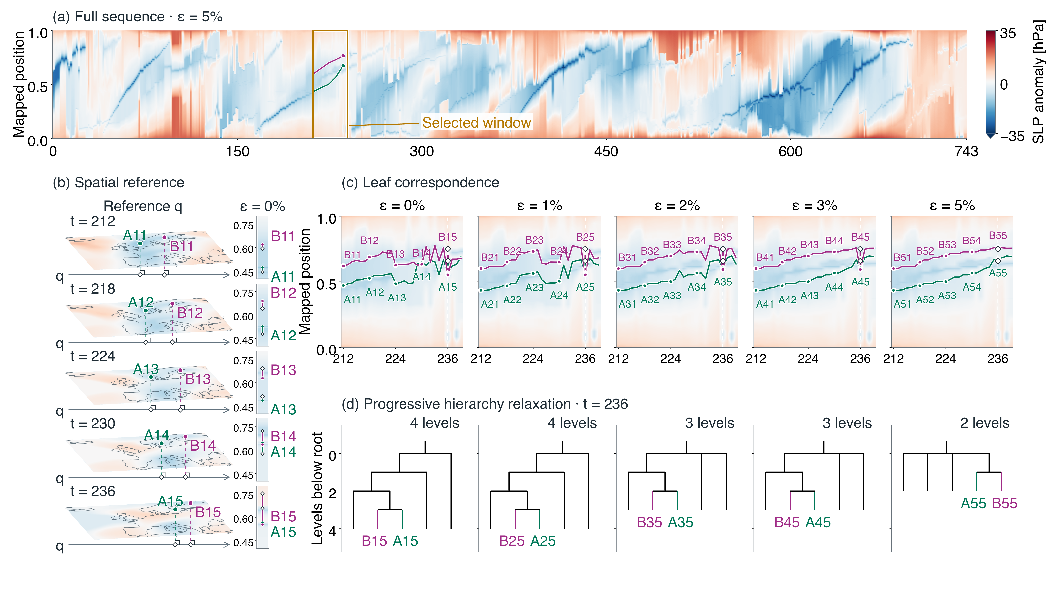
\includegraphics[width=\linewidth]{figures/fig_storms_hourly_ppt.pdf}
\par\smallskip\refstepcounter{figure}\label{fig:teaser}
{\captionfonts\noindent\figurename~\thefigure: Hourly Storms: 744 sea-level-pressure anomaly fields from December 1999. (a) Full map at $\varepsilon=5\%$; the box selects $t=212$--239. (b) Five spatial snapshots with the fixed reference axis $q$ and exact-layout positions. (c) The same tracked minima A (green) and B (magenta) at budgets $0,1,2,3,5\%$; diamonds mark references at the selected step. Labels $A_{ij},B_{ij}$ index parameter column $i$ and sampled time $j$. (d) Complete displayed trees at $t=236$: structural depths $4,4,3,3,2$. Roots are top-aligned; vertical distance counts levels below the root, not pressure. This hourly diagnostic is separate from the half-day Storms benchmark.\par}
}

\begin{document}
\firstsection{Introduction}
\maketitle

Static summaries of time-varying scalar fields show a whole sequence at once, without relying on memory across animation frames~\cite{Tversky:2002:Animation,Robertson:2008:Animation,Archambault:2011:AMM}. Merge tree maps build such summaries from topology~\cite{Koepp:2023:TMTM,STMTM:2026}. At each time step the merge tree of the field is linearized into a one-dimensional profile whose basins are the extrema and whose barriers are their merge levels; the profiles are stacked along time, so every feature becomes a band and the nesting of bands shows how features connect.

The cost of this compression is the meaning of the axis. Temporal Merge Tree Maps (TMTM) order features by a tree traversal aligned across time~\cite{Koepp:2023:TMTM}; Spatiotemporal Merge Tree Maps (ST-MTM) add pairwise distances~\cite{STMTM:2026}. Neither ties a feature to a coordinate the analyst already knows, and a feature can be drawn far from its spatial reference. Figure~\ref{fig:teaser} links spatial snapshots, mapped trajectories and the hierarchy across explicit budgets. Hovm\"oller diagrams make the opposite choice~\cite{Hovmoller:1949}: the axis is longitude, which is immediately readable, but the hierarchy is lost. This paper asks how close a merge tree map can come to both.

The question has a precise answer. If the merge tree is kept intact, every subtree occupies one contiguous block of the axis; two sibling subtrees whose reference ranges overlap cannot both stay at their references. We show that this conflict determines the unavoidable displacement in closed form, that it is attainable, and that most of the displacement of existing maps lies above it (Fig.~\ref{fig:teaser}c). When the analyst accepts a bounded change of merge levels, the same reasoning bounds how much position can be recovered, and the change is shown on the map.

Our contributions are:
\begin{itemize}
\item \textbf{Certified lower bounds} on the displacement of any merge tree map that keeps the hierarchy: a closed-form bound on the order error, valid for every method including TMTM and ST-MTM; a width-aware bound on the worst displacement for interval layouts such as ST-MTM and ours; and chain-aware bounds for maps with a merge-level budget $\varepsilon$ (Sect.~\ref{sec:bounds}). In 3-D, the order bound ranks candidate reference directions before any map is drawn.
\item \textbf{Layouts that attain them}: midpoint ordering, a width-aware search and a budgeted ordering with exact merge-cost checks, combined with optimal barriers and a capped quadratic placement; every map reports its position and merge-level errors and marks changed merges (Sect.~\ref{sec:method}).
\item \textbf{One formulation} with explicit position and topology budgets, in which TMTM and ST-MTM are exact-topology instances; given their own leaf orders, their layouts are reproduced exactly (Sect.~\ref{sec:background}).
\item \textbf{A cross-method comparison} of five methods on 917 frames from seven sequences, including two volumetric ones, a study of the reference direction in 3-D, and a case study with error disclosure (Sect.~\ref{sec:evaluation}).
\end{itemize}
We study faithfulness, not readability; a perceptual study is future work.

\section{Related Work}\label{sec:related}

\begin{figure*}[t]
\centering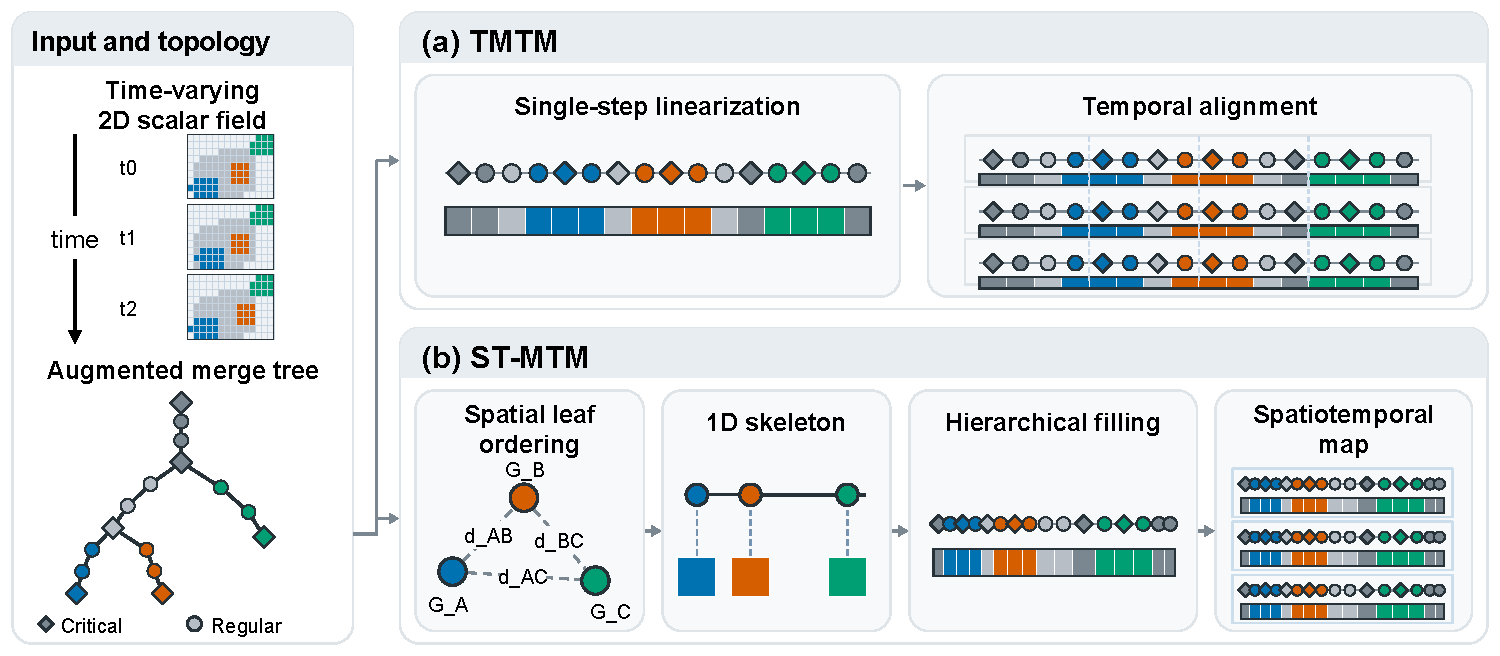
\includegraphics[width=.92\linewidth]{figures/fig_prior.pdf}
\caption{Existing merge tree map pipelines on a shared augmented merge tree. (a) TMTM linearizes each tree and aligns adjacent steps by subtree overlap. (b) ST-MTM orders leaves by spatial proximity, places a one-dimensional skeleton and fills it hierarchically. Neither uses an absolute spatial reference.}\label{fig:prior}
\end{figure*}

\paragraph{Linearizing space and time.}
Space--time cubes and their flattenings organize temporal visualization~\cite{Bach:2017:STC}. Hovm\"oller diagrams keep one spatial coordinate~\cite{Hovmoller:1949}; space-filling curves, geographic orderings and data-driven projections linearize the whole domain~\cite{Dafner:2000:CSFC,Guo:2006:SpatialOrder,Zhou:2021:DSF,Franke:2021:1DP,Weissenboeck:2019:DVL}, and MotionRugs and related summaries order moving entities~\cite{Buchmueller:2019:MR,Wulms:2021:SVS,Valdrighi:2024:MRV,Stolk:2025:GR}. None of them represents the merge hierarchy. Storyline layouts solve a related time$\times$1D problem, minimizing crossings and wiggles, partly by quadratic programming~\cite{Tanahashi:2012:Storyline,Liu:2013:SF,Dobler:2025:Wiggle}; their entities have neither a fixed coordinate nor nesting.

\paragraph{Drawing merge and contour trees.}
Topology-based visualization is surveyed by Heine et al.~\cite{Heine:2016:Survey}. Contour trees have been drawn in the plane~\cite{Heine:2011:DCT}, as terrains~\cite{Weber:2007:TL}, with geometry-preserving terrain layouts~\cite{Beketayev:2012:GPTL}, and as one-dimensional landscape profiles~\cite{Oesterling:2013:TLP}, which Herick et al.\ make temporally coherent~\cite{Herick:2020:TCTL}. Mergemaps argue that nesting is hard to read in profiles and use treemaps~\cite{Kamakshidasan:2021:MM}. TMTM introduced the time$\times$1D merge tree map~\cite{Koepp:2023:TMTM} and ST-MTM made it geometry-aware~\cite{STMTM:2026} (Fig.~\ref{fig:prior}). Tracking graphs show feature evolution without a spatial axis~\cite{Widanagamaachchi:2012:DTG,Lukasczyk:2017:NTG,Lukasczyk:2020:DNTG,Koepp:2019:TT,Oesterling:2017:TVMT}. We keep the TMTM/ST-MTM map and its renderer and change what the layout optimizes; our bounds apply to all such profile layouts.

\paragraph{Ordering the leaves of a tree.}
Optimal leaf ordering selects one of the $2^{n-1}$ tree-consistent orders to minimize adjacent dissimilarity~\cite{BarJoseph:2001:OLO,Eisen:1998:CA}. Closest to our question are reordering a tree towards a given leaf order~\cite{Bulteau:2022:RT} and one-sided tanglegrams~\cite{Fernau:2010:CTC,Dobler:2026:BCT,Huson:2026:DOT}; geophylogenies combine tree constraints with map positions~\cite{Klawitter:2025:GP}. These works count inversions, crossings or summed displacement; minimizing the number of inversions against a target order is NP-complete for trees of unbounded degree~\cite{Bulteau:2022:RT}. We measure the \emph{maximum} displacement in reference units, which has a closed form, and extend it to interval widths, anchor slack and controlled violations of the tree.

\paragraph{Ordered merge trees and distances.}
A merge tree with a leaf order is equivalent to a one-dimensional curve; Beurskens et al.\ define a monotone interleaving distance for such ordered merge trees~\cite{Beurskens:2025:OMT}, visualized by ParkView~\cite{Beurskens:2025:ParkView}. For labelled merge trees, the $\ell_\infty$ distance between cophenetic matrices is an interleaving distance~\cite{Munch:2019:LINF}, used as the labelled interleaving distance~\cite{Gasparovic:2024:IID}; it bounds the unlabelled interleaving distance~\cite{Gasparovic:2024:IID}, which bounds the bottleneck distance of persistence diagrams~\cite{Morozov:2013:IDMT}. Geometry-aware and Wasserstein comparisons extend these distances~\cite{Yan:2022:GAMT,Pont:2022:WMT,Yan:2021:Survey}. Fitting an ultrametric under $\ell_\infty$ error has a closed form~\cite{Farach:1995:RM}; our optimal barriers are such a fit under a fixed leaf order.

\section{Background and Problem}\label{sec:background}

\begin{figure*}[t]
\centering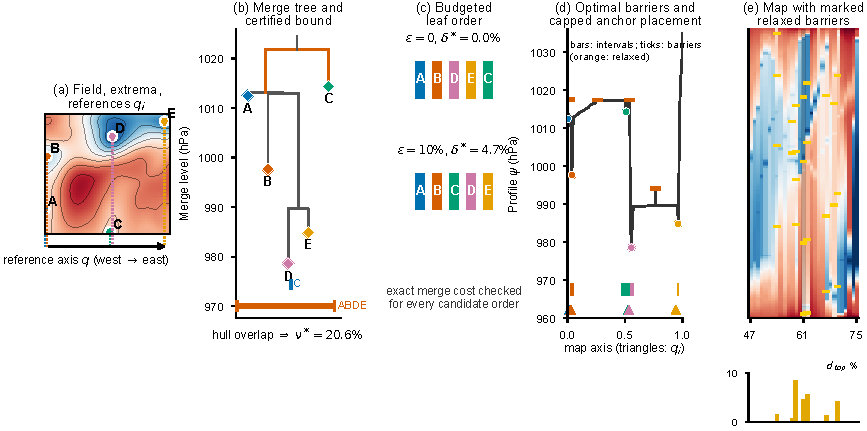
\includegraphics[width=\linewidth]{figures/fig_pipeline.pdf}
\caption{Our pipeline on one Storms step (17 Dec 1999, 12 UTC). (a) Extrema and references. (b) Merge tree; the root's children $\{C\}$ and $\{A,B,D,E\}$ have overlapping reference hulls (bars below), which certifies $\nu^*=20.6\%$ for every exact map. (c) Leaf orders at $\varepsilon=0$ and $10\%$ with their exact merge cost $\delta^*$. (d) Profile with optimal barriers (ticks; orange where the merge level was changed), intervals (bars), anchors (dots) and references (triangles). (e) Map around this step with marked barriers and the per-step merge error.}\label{fig:pipeline}
\end{figure*}

\paragraph{Merge tree maps.}
A sequence of scalar fields $f_t$ on a two- or three-dimensional domain gives, per time step, a merge tree $T_t$ of its sublevel (or superlevel) sets. Its leaves are the $n_t$ retained extrema; $V_{ij}$ is the level at which leaves $i$ and $j$ merge, the value of $\lca(i,j)$, and $\Delta_F$ is the scalar range. Features are matched across time by support overlap. Figure~\ref{fig:prior} shows the two existing pipelines. TMTM linearizes the augmented merge tree by a depth-first traversal and flips subtrees greedily to maximize the overlap of subtree intervals between adjacent steps~\cite{Koepp:2023:TMTM}. ST-MTM orders leaves by spatial proximity, places a one-dimensional skeleton by a quadratic program on pairwise distances, and fills it hierarchically~\cite{STMTM:2026}. A map frame is $M_t=(\pi_t,x_t,\psi_t)$: a leaf order, anchor positions and a profile $\psi_t:[0,L]\to\mathbb{R}$. As in ST-MTM, leaf $i$ occupies an interval of width $W_i=s\,m_i$ proportional to its support measure $m_i$, intervals are separated by a gap $g$, and the anchor (the basin extremum) lies within $H_i=\rho W_i/2$ of the interval centre.

\paragraph{References.} Each leaf has a reference coordinate $q_i\in[0,L]$, the projection of its location onto a fixed world direction, constant over time; $L$ is the canvas length in world units. On the Storms benchmark the direction is west--east; the hourly diagnostic uses a fixed projected direction (Fig.~\ref{fig:teaser}b); on Tangaroa it is the principal direction of matched feature motion, and on Cylinder the streamwise axis. Any fixed one-dimensional quantity, such as distance to a site, can serve. Nothing below depends on the dimension of the domain: the bounds use only the tree, the references and the widths.

\paragraph{Errors.} \emph{Position}: the displacement $|x_i-q_i|/L$, pooled over leaves and frames ($E_{\mathrm{pool}}$) and its maximum ($E_\infty$). \emph{Order}: the reference-order error of a leaf order,
\begin{equation}\label{eq:nroe}
\nroe(\pi)=\frac{1}{2L}\max_{k}\Big(\max_{j\le k} q_{\pi(j)}-q_{\pi(k)}\Big),
\end{equation}
the smallest worst displacement of any monotone placement in that order with zero widths; it is scale-free and therefore also compares maps without a world canvas. \emph{Topology}: in the profile, leaves $i,j$ merge at the highest value of $\psi_t$ between their anchors, $V^\psi_{ij}$, and
\begin{equation}\label{eq:dtop}
\dtop(\psi_t,T_t)=\max_{i,j}\big|V^{\psi}_{ij}-V_{ij}\big|,\qquad \mathrm{NMLE}=\dtop/\Delta_F .
\end{equation}
Labelling every extremum and its anchor by its feature, $V$ and $V^\psi$ are the cophenetic matrices of two labelled merge trees (diagonal $V_{ii}=f(i)$, which the profile keeps), so $\dtop$ is their labelled interleaving distance~\cite{Gasparovic:2024:IID,Munch:2019:LINF}. It requires the labels to cover all leaves, i.e., no unlabelled extremum in the profile; every rendered column we checked satisfies this. Hence $d_B\le d_I\le\dtop$~\cite{Gasparovic:2024:IID,Morozov:2013:IDMT}: a map with $\dtop\le\varepsilon\Delta_F$ displays a tree, and a persistence diagram, within $\varepsilon\Delta_F$ of the source. For superlevel sets all statements apply to $-f$.

\paragraph{One problem.} All maps we consider solve, per sequence,
\begin{equation}\label{eq:problem}
\begin{aligned}
\min_{\{M_t\}}\ &\textstyle\sum_t \lambda_O E_O+\lambda_G E_G+\lambda_M E_M+\lambda_R E_R+\lambda_W E_W\\
\text{s.t. }&M_t\in\mathcal{L}(\pi_t),\quad \|x_t-q_t\|_\infty\le B_t,\\
&\dtop(\psi_t,T_t)\le(\varepsilon_0+\varepsilon)\Delta_F ,
\end{aligned}
\end{equation}
with the TMTM overlap term $E_O$, the stress $E_G$ of anchor distances against source distances, a temporal term $E_M$ on matched anchors, the reference error $E_R$, the width deviation $E_W$ and layout model $\mathcal{L}$ (notation in Table~\ref{tab:notation}). The data resolution $\varepsilon_0$ treats merge levels closer than $\varepsilon_0\Delta_F$ as ties (float32 round-off); $\varepsilon$ is the budget the analyst spends and $B_t$ a position cap. Table~\ref{tab:instances} lists the methods we compare as instances. Given their native leaf orders, both previous layouts are reproduced exactly on all five planar sequences: the TMTM linearization equals the official implementation in all 3127 arc intervals and anchors, and the ST-MTM anchors satisfy the optimality conditions of its quadratic programs (relative KKT residuals below $10^{-6}$, below $10^{-10}$ on the volumetric sequences). Both methods are heuristic in the order: ST-MTM's leaf ordering exceeds the exhaustive optimum of its own objective on 10 frames, and TMTM's greedy choice is optimal at 434 of 463 enumerated steps but up to 85.5\% above the per-step optimum elsewhere. The bounds below depend only on the shared constraints.

\begin{table}[t]
\caption{Notation.}\label{tab:notation}
\centering\scriptsize\setlength{\tabcolsep}{3pt}
\begin{tabular}{ll}\toprule
Symbol & Meaning\\\midrule
$T_t$, $V_{ij}$, $\Delta_F$ & merge tree of step $t$, merge level of leaves $i,j$, scalar range\\
$q_i$, $L$ & reference coordinate of leaf $i$, canvas length\\
$W_i$, $g$, $H_i$ & interval width, gap between intervals, anchor slack $\rho W_i/2$\\
$\pi_t$, $x_i$, $\psi_t$ & leaf order, anchor position, profile of step $t$\\
NROE, $\tau$ & reference-order error (Eq.~\ref{eq:nroe}); attained worst displacement\\
$\dtop$, NMLE & labelled merge error (Eq.~\ref{eq:dtop}); $\dtop/\Delta_F$\\
$\nu^*$ & lower bound on NROE for exact maps (Theorem~\ref{thm:order})\\
$\varepsilon$, $\varepsilon_0$, $B_t$ & merge-level budget, data resolution, position cap\\
$\delta^*(\pi)$ & smallest merge error of order $\pi$ (optimal barriers)\\\bottomrule
\end{tabular}
\end{table}

\begin{table}[t]
\caption{Methods compared, as instances of problem~(\ref{eq:problem}).}\label{tab:instances}
\centering\scriptsize\setlength{\tabcolsep}{2.5pt}
\begin{tabular}{lcccl}\toprule
Method & $\varepsilon$ & $B$ & objective & solver\\\midrule
TMTM~\cite{Koepp:2023:TMTM} & 0 & $\infty$ & $E_O$ & greedy subtree flips\\
ST-MTM~\cite{STMTM:2026} & 0 & $\infty$ & $E_G+\lambda E_M$; $E_W$ & leaf order, then QP\\
$\kappa$ R20 (earlier) & uncapped & -- & $E_R+E_G+E_M$ & candidate pool + QP\\
Projection & $\infty$ & $\tau_t+\beta$ & -- & sort by $q$ + QP\\
Ours & 0 or $\varepsilon$ & $\tau_t+\beta$ & $E_R+E_G+E_M$ & Algorithm~\ref{alg:layout}\\\bottomrule
\end{tabular}
\end{table}

\section{Overview}\label{sec:overview}
Figure~\ref{fig:pipeline} follows one Storms time step through our pipeline. (a) The extrema of the field are projected onto the reference axis. (b) Their merge tree is fixed by the data. Minimum C joins the other four only at the root, so any exact map keeps A, B, D, E in one block and places C at one of its ends; since C's reference lies inside the range of that block, the order error is at least $\nu^*=20.6\%$ (Theorem~\ref{thm:order}). (c) With a budget $\varepsilon=10\%$, the budgeted ordering moves C next to D, near its reference, at an exact merge cost $\delta^*=4.7\%$. (d) Optimal barriers realize this order with the smallest possible merge error, and a capped quadratic program places the anchors. (e) The stacked map marks every barrier whose displayed merge level was changed, and a strip reports the merge error spent per step.

\section{Certified Bounds}\label{sec:bounds}
All bounds follow from one lemma about where a leaf may sit.

\begin{figure}[t]
\centering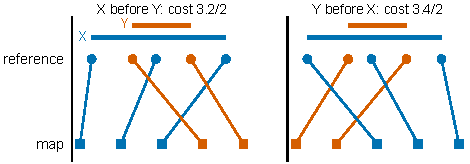
\includegraphics[width=\columnwidth]{figures/fig_concept.pdf}
\caption{Theorem~\ref{thm:order} on sibling subtrees $X$ (blue) and $Y$ (orange). With exact topology one block must precede the other; the cheaper orientation costs $\min(M_X-m_Y,M_Y-m_X)/2$ and is chosen by sorting hull midpoints.}\label{fig:concept}
\end{figure}

\begin{lemma}[Separation]\label{lem:sep}
Let $u$ be a node of $T_t$ with level $f(u)$, and let leaf $k$ lie strictly between two leaves $i,j$ of $u$ in a map with $\dtop\le\varepsilon$. Then $V_{ik}\le f(u)+2\varepsilon$.
\end{lemma}
\begin{proof}
The displayed merge of $i,j$ is the highest profile value between them, which is at least the displayed merge of $i,k$. Hence $V_{ik}-\varepsilon\le V^\psi_{ik}\le V^\psi_{ij}\le V_{ij}+\varepsilon\le f(u)+\varepsilon$.
\end{proof}

With $\varepsilon=0$, a leaf outside $u$ merges with $u$ strictly above $f(u)$, so \emph{every subtree is contiguous}: the children of a node occupy disjoint blocks. Let $[m_X,M_X]$ be the reference hull of a subtree $X$.

\begin{theorem}[Order bound]\label{thm:order}
Every map with $\dtop=0$ satisfies
\begin{equation}\label{eq:nu}
\begin{aligned}
\nroe(\pi_t)\ &\ge\ \nu^*(T_t)\\
&=\frac{1}{2L}\max_{v}\ \max_{X\ne Y\in\mathrm{ch}(v)}\big[\min(M_X-m_Y,\ M_Y-m_X)\big]^+ ,
\end{aligned}
\end{equation}
and sorting the children of every node by hull midpoint attains the bound in $O(n\log n)$.
\end{theorem}
\begin{proof}
If $X$ precedes $Y$, the leaf of $X$ at $M_X$ precedes the leaf of $Y$ at $m_Y$, which by (\ref{eq:nroe}) costs at least $(M_X-m_Y)/2L$; the other orientation costs $(M_Y-m_X)/2L$. In a midpoint order every inverted pair lies in sibling blocks $X\prec Y$ of its lowest common ancestor, and $m_X+M_X\le m_Y+M_Y$ is exactly $M_X-m_Y\le M_Y-m_X$.
\end{proof}

The bound is geometric (Fig.~\ref{fig:concept}): siblings pay in proportion to how deeply their reference hulls overlap. It holds for any width rule, layout model or solver, hence for TMTM and ST-MTM. The width-aware bound below needs the interval model, which ST-MTM and our layouts share.

\paragraph{Widths.} A wide feature pushes its neighbours away. The attained interval cost $\tau(\pi)=\min_{x\in\mathcal{L}(\pi)}\max_i|x_i-q_i|$ has a closed form over the packed intervals. With $\ell_k=q_k-W_k/2-H_k$, $h_k=q_k+W_k/2+H_k$, $s_k=W_k+g$ and, for a leaf set $S$,
\begin{equation}
A(S)=\max_{\alpha}\Big[\alpha+\!\!\sum_{k\in S,\ \ell_k\ge\alpha}\!\! s_k\Big],\quad
B(S)=\max_{\beta}\Big[\sum_{k\in S,\ h_k\le\beta}\!\! s_k-\beta\Big],
\end{equation}

\begin{theorem}[Width-aware bound]\label{thm:width}
In the interval layout model, if block $X$ precedes block $Y$, then $\tau\ge (A(X)+B(Y)-g)/2$. Hence every exact interval layout has $\tau(\pi_t)\ge\max_v\max_{X\ne Y\in\mathrm{ch}(v)}\frac12[\min(A(X)+B(Y),A(Y)+B(X))-g]$, and every map has $\tau\ge B(\text{all})-g$ and $\tau\ge A(\text{all})-g-L$ at the canvas ends.
\end{theorem}
\begin{proof}[Proof sketch]
For $S_X\subseteq X$, $S_Y\subseteq Y$, the first interval of $S_X$ and the last of $S_Y$ enclose all of $S_X\cup S_Y$; their anchors are thus at least $\sum_{S_X\cup S_Y}s_k-g-W_a/2-W_b/2-H_a-H_b$ apart, and $\tau$ is at least half the shortfall against $q_a-q_b$. Upper sets of $\ell$ and lower sets of $h$ separate the maximization into $A$ and $B$, computed by sorting and prefix sums. The full proof is in the supplement.
\end{proof}
With zero widths and gap, Theorem~\ref{thm:width} reduces to $L\,\nu^*$.

\paragraph{A merge-level budget.} With $\dtop\le\varepsilon$, Lemma~\ref{lem:sep} still forbids a leaf between two leaves of $u$ unless it merges with $u$ within $2\varepsilon$ of $f(u)$. Let $A_\varepsilon(u)$ be the highest ancestor of $u$ with level at most $f(u)+2\varepsilon$.

\begin{theorem}[Chain bounds]\label{thm:chain}
In a map with $\dtop\le\varepsilon$, every leaf outside $A_\varepsilon(u)$, and every node $w$ with $w\notin A_\varepsilon(u)$ and $u\notin A_\varepsilon(w)$, lies entirely on one side of $u$. Applying the argument of Theorem~\ref{thm:order} (resp.\ \ref{thm:width}) to these separated pairs bounds NROE (resp.\ $\tau$) from below.
\end{theorem}
A coarser bound flattens every node within $2\varepsilon$ of its parent and applies Theorems~\ref{thm:order} and~\ref{thm:width}; the chain bound charges a chain of small gaps by their sum and is never weaker. All bounds use $\varepsilon_0+\varepsilon$ when a data resolution is declared. Full proofs are in the supplement; every bound was checked against exhaustive enumeration on random trees.

\begin{figure}[t]
\centering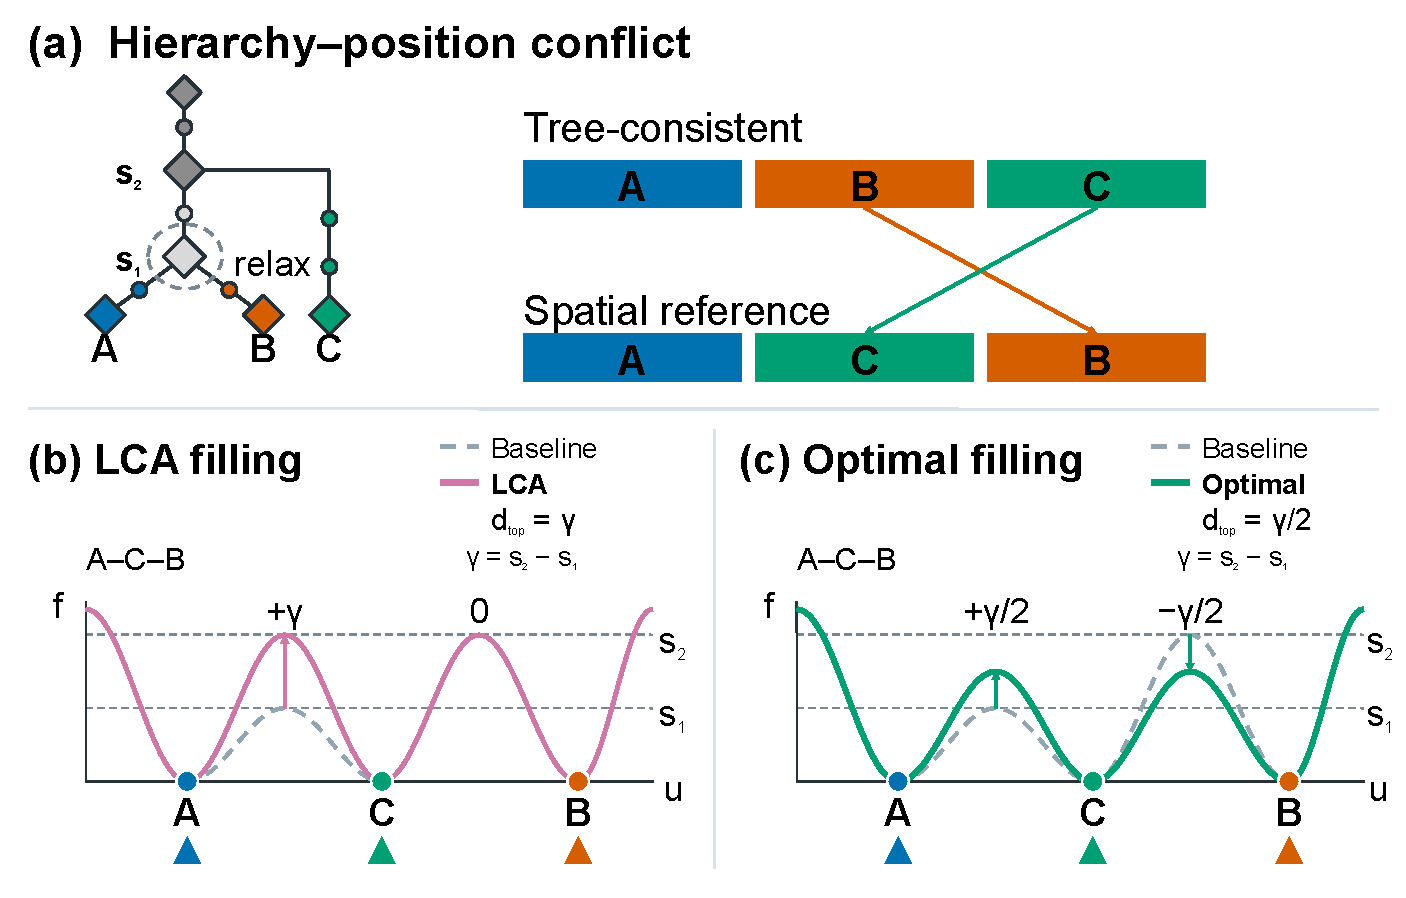
\includegraphics[width=\columnwidth]{figures/fig_conflict.pdf}
\caption{(a) Reference order A--C--B splits the subtree A--B. (b) Filling barriers with the original lowest-common-ancestor levels errs by the full gap $\gamma$. (c) Optimal barriers balance the error at $\gamma/2$, the minimum for this order.}\label{fig:conflict}
\end{figure}

\section{Certified Layouts}\label{sec:method}

\begin{figure*}[t]
\centering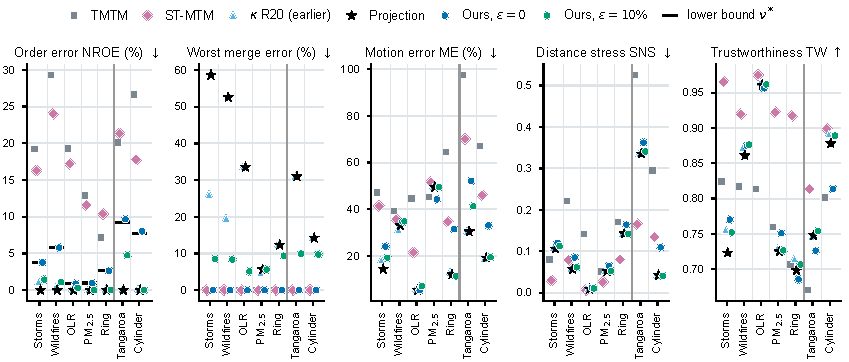
\includegraphics[width=\linewidth]{figures/fig_compare.pdf}
\caption{Cross-method comparison on seven sequences (left of the grey line: planar; right: volumetric). Order error with the certified lower bound $\nu^*$ (black ticks; no exact map can go below), worst merge error, motion error, and the two distance measures of ST-MTM. Exact-topology methods (TMTM, ST-MTM, ours at $\varepsilon=0$) have zero merge error; the projection has zero order error but up to 59\% merge error. Values are in the supplement.}\label{fig:compare}
\end{figure*}




Algorithm~\ref{alg:layout} computes one map frame; frames are processed in time order so that the temporal term refers to the previous frame.

\begin{algorithm}[t]
\caption{Certified map frame $t$}\label{alg:layout}
\small
\begin{algorithmic}[1]
\Require tree $T_t$, references $q$, widths $W$, budget $\varepsilon$, resolution $\varepsilon_0$, slack $\beta$, previous anchors $x_{t-1}$
\State $\mathcal{S}\gets\{T_t\}\cup\{T_t^{(s)}: s\le 2(\varepsilon_0+\varepsilon)\}\cup\{\text{conflict-driven flattening}\}$ \Comment{candidate trees}
\For{$S\in\mathcal{S}$}
  \State $\pi\gets$ midpoint order of $S$; \textbf{skip} if $\delta^*(\pi)>(\varepsilon_0+\varepsilon)\Delta_F$
  \Repeat \Comment{width-aware local search}
    \State move one child block of a node of $S$ if it lowers $(\tau,\ \textstyle\sum\text{positive terms}^2)$ and $\delta^*\le(\varepsilon_0+\varepsilon)\Delta_F$
  \Until{no move improves}
\EndFor
\State $\pi_t\gets$ best order by $(\tau,\nroe)$ \Comment{includes the point-model order}
\State barriers $\gets$ optimal barriers of $\pi_t$, attaining $\delta^*(\pi_t)$
\State $x_t\gets\arg\min E_R+E_G+E_M$ s.t.\ $\mathcal{L}(\pi_t)$, $\|x-q\|_\infty\le\tau(\pi_t)+\beta$
\State report lower bound, $\tau(\pi_t)$, $\delta^*(\pi_t)$; mark barriers changed by more than $10^{-3}\Delta_F$
\end{algorithmic}
\end{algorithm}

\paragraph{Ordering.} For $\varepsilon=0$, midpoint ordering attains $\nu^*$. With widths, a local search over the child permutations of each node minimizes $\tau$; the sum of squared positive pair terms breaks plateaus of the minimax objective. Every child permutation of the exact tree keeps $\dtop=0$. For $\varepsilon>0$, candidate trees flatten nodes either by threshold or by repeatedly releasing the sibling pair that sets the order cost when Theorem~\ref{thm:chain}'s chain condition allows; every candidate and every search move is checked with the exact merge cost $\delta^*$ and rejected if it exceeds the budget. The best previous order is always kept, so refinement never increases $\tau$.

\paragraph{Search details.} Threshold candidates use one tree per distinct parent gap up to $2(\varepsilon_0+\varepsilon)$. The conflict-driven candidate starts from the exact tree, finds the sibling pair with the largest order cost and flattens one or both of its nodes when the chain condition holds and the exact $\delta^*$ of the new midpoint order stays within the budget; it repeats while the order error does not increase. The four candidates with the lowest initial $\tau$, together with the exact tree, are refined. A move reinserts one child block at another position among its siblings, over all positions for nodes with up to eight children and within distance three otherwise, for at most eight passes. On 300 random trees with random widths and budgets, this search reached the exhaustive optimum of $\tau$ on 296; the point-model order alone on 250.

\paragraph{Optimal barriers.} For a fixed order, the barrier between consecutive basins determines every displayed merge. The smallest achievable error $\delta^*(\pi)$ has a closed form: each pair is limited by the lowest true merge level among the pairs it separates, an $\ell_\infty$ ultrametric fit under a fixed leaf order~\cite{Farach:1995:RM}. Figure~\ref{fig:conflict} shows the effect: keeping original merge levels doubles the error that a balanced barrier needs. The profile is filled from the source arc samples with the renderer of ST-MTM~\cite{STMTM:2026}.

\paragraph{Capped placement.} The anchors solve the convex quadratic program of~(\ref{eq:problem}) with widths, gaps, canvas and anchor slack. The cap $B_t=\tau(\pi_t)+\beta$ is feasible because $\tau$ is attained by the order, and it bounds $E_\infty$; without it the geometry term can pull single anchors far from their references.

\paragraph{Cost.} Bounds cost $O(n\log n)$ to $O(n^2\log n)$, $\delta^*$ $O(n^3)$ per order. On an Apple M2 Pro (single Python process; NumPy 2.0, SciPy 1.13), all bounds take at most 0.6\,ms per planar frame (1--11 leaves) and 5.5\,ms per volumetric frame (up to 93 leaves), the ordering at most 3.7\,ms and 103\,ms, and the capped QP (SciPy SLSQP) 2.3--9.0\,ms and 0.25--0.50\,s. All 917 frames take 94\,s at $\varepsilon=0$ and at most 137\,s with a budget.

\section{Evaluation}\label{sec:evaluation}

\begin{figure*}[t]
\centering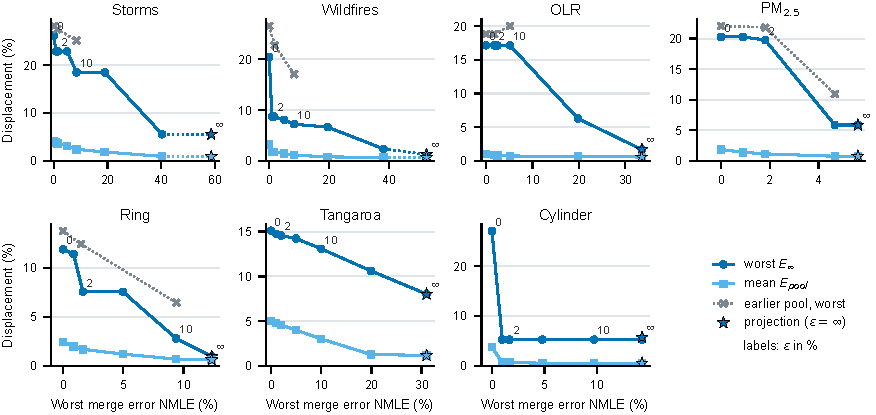
\includegraphics[width=\linewidth]{figures/fig_frontier.pdf}
\caption{Position--topology frontier per sequence. Each point is one layout of all frames at budget $\varepsilon$ (labels, in percent), placed by its measured worst merge error and its worst (dark) and mean (light) displacement. Stars: projection ($\varepsilon=\infty$). Grey crosses: earlier candidate-pool QP, planar only.}\label{fig:frontier}
\end{figure*}

\subsection{Setup}
\paragraph{Data.} Table~\ref{tab:data} lists seven sequences, 917 frames in total~\cite{Hersbach:2020:ERA5,Franke:2021:1DP,NOAA:OLR,Dong:2026:PM25,Koepp:2023:TMTM,Popinet:2004:Tangaroa,Camarri:2005:Cylinder,Weinkauf:SquareCylinder}. All methods share the processed fields, extrema, supports, matches and references; preprocessing follows prior work.

\begin{table}[t]
\caption{Sequences. Leaves: retained extrema per frame.}\label{tab:data}
\centering\scriptsize\setlength{\tabcolsep}{3pt}
\begin{tabular}{llrrl}\toprule
Sequence & Scalar field & Frames & Leaves & Tree\\\midrule
Storms & ERA5 mean sea-level pressure, 2-D & 118 & 1--8 & join\\
Wildfires & $\log(1+\mathrm{FRP})$, 2-D & 30 & 6--11 & split\\
OLR & outgoing longwave radiation, 2-D & 60 & 2--8 & join\\
PM$_{2.5}$ & PM$_{2.5}$ concentration, 2-D & 366 & 1--7 & split\\
Ring & synthetic ring intensity, 2-D & 40 & 1--7 & split\\
Tangaroa & velocity magnitude, 3-D & 201 & 18--93 & join\\
Cylinder & Q criterion, 3-D & 102 & 4--75 & split\\\bottomrule
\end{tabular}
\end{table}

\paragraph{Methods and metrics.} We compare native TMTM and ST-MTM outputs, the earlier uncapped $\kappa$ construction (R20), the projection baseline, which sorts every frame by reference and uses the same optimal barriers and capped QP, and our layouts at $\varepsilon=0$ and $10\%$ (Table~\ref{tab:instances}), with $\varepsilon_0=10^{-7}$. Metrics are the order error NROE, the worst merge error, and, with the protocol of ST-MTM~\cite{STMTM:2026}, scale-normalized stress (SNS) and trustworthiness (TW, $k=1$) of anchor distances against support-centroid distances, and the motion error (ME): the fraction of clear approach or separation events between two features over two steps that the map shows in the wrong direction or not at all. Recomputing the stored baseline values from their saved anchors reproduces SNS and TD to a relative $10^{-5}$ and TW and ME to the third decimal or one event.

\subsection{Cross-method comparison}\label{sec:compare}

\takeaway{Exact-topology maps can be far more position-faithful than existing ones; the remaining error is certified, and distance preservation is a different trade-off.}
Figure~\ref{fig:compare} compares all methods on all sequences. \emph{Order}: no method falls below $\nu^*$ on any of the 917 frames. Most of the order error of TMTM and ST-MTM is avoidable: on Storms, TMTM's 19.2\% contains 3.8\% that the hierarchy forces and ST-MTM's 16.3\% contains 12.5\% that it does not. Our exact layouts lie within 0.03 percentage points of $\nu^*$ on every planar sequence; on Tangaroa and Cylinder the width-aware order trades a little NROE (9.67\% against 9.24\% on Tangaroa) for a lower worst displacement. On all 637 frames with at most eight leaves, the budgeted order matches exhaustive enumeration at nine budgets from 0 to 100\%. \emph{Topology}: the projection has zero order error but changes merge levels by up to 58.66\% of the scalar range on Storms, 52.58\% on Wildfires, 33.56\% on OLR and 31.02\% on Tangaroa, where no frame keeps its tree; the uncapped $\kappa$ construction reached the same worst values on OLR and Tangaroa. Our budgeted maps never exceed their budget. \emph{Motion}: our exact maps make fewer motion errors than both TMTM and ST-MTM on all seven sequences, e.g., 5.4\% against 21.4\% on OLR and 52.2\% against 70.0\% on Tangaroa, because a feature that moves along the reference moves on the map; the projection, which follows the references exactly, is lowest on most sequences. \emph{Distance}: ST-MTM, which optimizes pairwise distances, has the best TW on all seven sequences and the best SNS on five; on Cylinder our budgeted map (0.041) and the $\kappa$ construction (0.040) are far below ST-MTM's 0.135.

The supplementary map comparison shows the planar sequences OLR and Ring with the same renderer and widths. On Ring, the TMTM-type objective keeps all features near the centre of the axis and the ST-MTM-type objective spreads them by pairwise distance; both place them far from their references, whereas our exact layout follows them and a 10\% budget changes the map only locally. On OLR, our exact map already places the low-radiation basins near their references, which makes it comparable to a time--longitude plot while keeping each basin's nesting.

\subsection{Controlled hierarchy conflict}\label{sec:controlled}
\begin{figure}[t]
\centering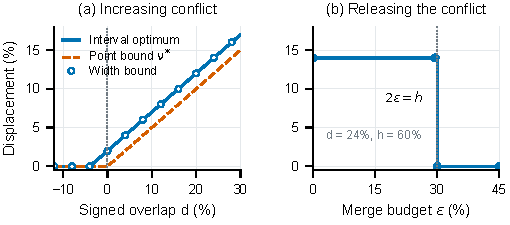
\includegraphics[width=\columnwidth]{figures/fig_controlled_conflict.pdf}
\caption{Controlled four-leaf trees. (a) Increasing sibling-hull overlap forces displacement; circles mark the width bound, attained by the exhaustive interval optimum. (b) At overlap $d=24\%$, the $14\%$ interval displacement disappears only when the merge budget reaches half the parent gap $h=60\%$. All percentages use a unit canvas or unit scalar range.}\label{fig:controlled}
\end{figure}
To isolate spatial conflict, we fix two sibling pairs $X=\{A,B\}$ and $Y=\{C,D\}$, merging at $0.4$ below a root at $1$, with leaf values $0$. On a unit canvas their references are $(0.2,0.5,0.5-d,0.8-d)$; signed overlap $d$ varies from $-0.12$ to $0.30$. Across 43 overlaps and four widths, we enumerate all 24 leaf orders and solve independent minimax placement LPs. The point optimum is exactly $\nu^*=\max(0,d)/2$. With equal widths $W=0.06$, gap $0.01$ and $\rho=0.5$, both the width bound and our search attain the exhaustive optimum $\tau=\max(0,(d+0.04)/2)$ (Fig.~\ref{fig:controlled}a). At $d=0.24$, these costs are $12\%$ and $14\%$. Sweeping the budget and four parent gaps confirms that interleaving becomes feasible at $2\varepsilon=h$; the $h=0.6$ case reaches zero displacement at $\varepsilon=0.3$ (Fig.~\ref{fig:controlled}b). These are controlled instances, not a general tightness claim for the width bound; full settings and packing costs are in the supplement.

\subsection{The position--topology frontier}
\takeaway{Small budgets can recover most of the position, but not on every sequence; the frontier shows where.}
Figure~\ref{fig:frontier} places every layout by its measured worst merge error and its displacement, from $\varepsilon=0$ to the projection. On Cylinder a 1\% budget reaches the lowest worst displacement of the whole curve (27.00\% to 5.27\%), below the projection's 5.73\%, because sorting by reference ignores widths. On Wildfires 1\% reduces $E_\infty$ from 20.48\% to 8.71\%, and on PM$_{2.5}$ 5\% reaches the projection result. Storms needs much more: its worst displacement stays above 18\% up to $\varepsilon=20\%$, and OLR keeps $E_\infty=17.14\%$ up to 10\% because one frame needs a larger change. Mean merge errors are far below the maxima (Storms at 10\%: 0.90\% mean, 8.51\% maximum), so the budget is spent on few frames. Compared with the uncapped $\kappa$ construction at similar positions, the worst merge error is now bounded (Storms: 26.07\% to 8.51\%; Wildfires: 19.56\% to 8.35\%).

\paragraph{Local budget response.} Aggregate gains do not imply pointwise improvement. In a four-leaf control, enumerating all 24 orders lowers the optimal worst displacement from 22\% to 1\% at $\varepsilon=30\%$, yet one feature's error rises from 0.087\% to 1\%. On an additional 90-frame Vortex diagnostic, increasing $\varepsilon$ from 20\% to 30\% lowers pooled error from 8.79\% to 4.27\%, while 30.91\% of 12,446 feature--frame observations worsen; 24.72\% worsen by at least 0.5 percentage points of $L$. Supplement S4 gives the fixed-population protocol, an hourly Storms check and local-response figures. These cohorts are separate from the 917-frame benchmark.

\subsection{Wide features}

\begin{figure*}[t]
\centering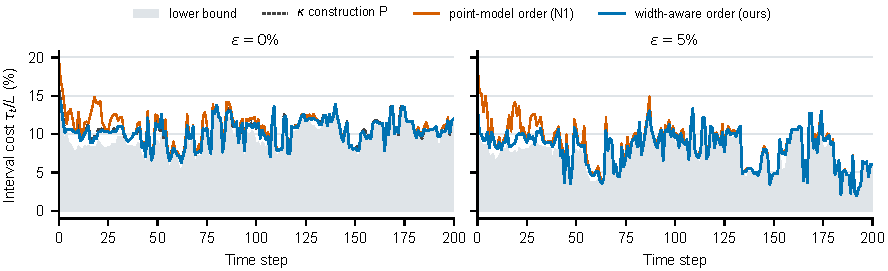
\includegraphics[width=\linewidth]{figures/fig_tangaroa.pdf}
\caption{Tangaroa, 201 time steps: interval cost $\tau_t/L$ of the point-model order (orange), the width-aware order (blue) and the $\kappa$ construction (dashed, mostly hidden under the blue line), with the certified lower bound (grey area, the larger of Theorems~\ref{thm:width} and~\ref{thm:chain}).}\label{fig:tangaroa}
\end{figure*}

\begin{figure*}[t]
\centering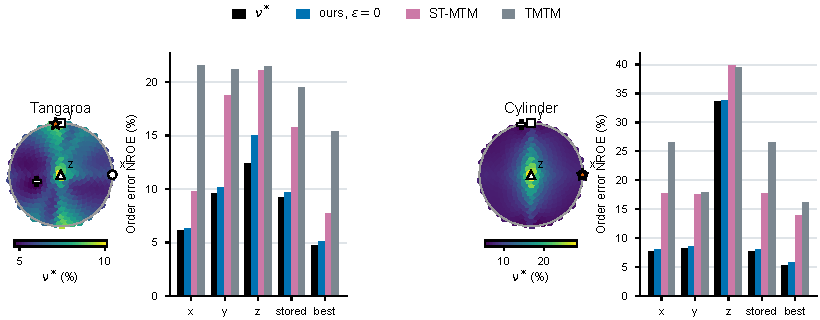
\includegraphics[width=\linewidth]{figures/fig_direction.pdf}
\caption{Reference direction in 3-D. Disks: mean order bound $\nu^*$ over 400 directions of the hemisphere (equal-area projection; centre $=z$, rim $=xy$ plane); markers: coordinate axes, stored direction (star) and smallest bound (cross). Bars: $\nu^*$ and mean order error of our exact layout, ST-MTM and TMTM for the key directions (native orientations chosen in their favour).}\label{fig:direction}
\end{figure*}

\begin{figure*}[t]
\centering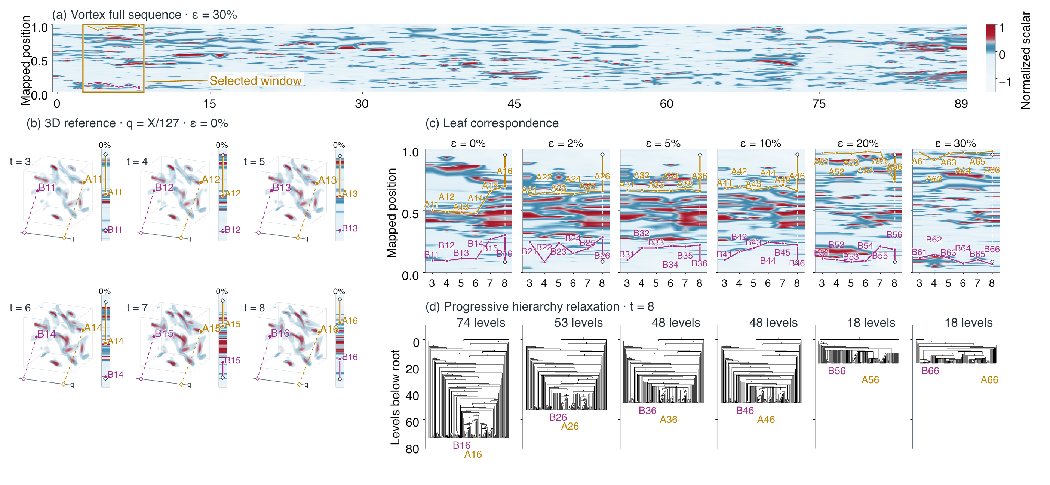
\includegraphics[width=\linewidth]{figures/fig_vortex_3d_ppt.pdf}
\caption{Vortex, 90 normalized $128^3$ volumes. (a) Full map at $\varepsilon=30\%$ and selected window. (b) Frames $t=3$--8 with orthogonal projections to $q=X/127$; diamonds indicate references and the adjacent strips use $\varepsilon=0$. (c) The same two tracked features at budgets $0,2,5,10,20,30\%$. Label digits index parameter column and time sample. (d) Complete displayed trees at $t=8$, all with 142 leaves, have structural depths $74,53,48,48,18,18$. Roots are top-aligned; the vertical axis counts levels below the root, not scalar differences.}\label{fig:vortexcase}
\end{figure*}

\takeaway{Ordering for the point model is not enough when features are large; the width-aware bound and search close the gap.}
On Tangaroa, ordering by NROE alone gave a worst displacement of 20.69\%, above the $\kappa$ construction's 16.86\%. Ordering by $\tau$ lowers it to 15.10\% at $\varepsilon=0$ and to 14.55\% at $\varepsilon=2\%$, where the worst frame meets the lower bound; on Cylinder $\varepsilon\ge2\%$ lowers $E_\infty$ from 5.73\% to 5.27\%, again at the bound. The chain bound makes these certificates informative for large trees: at $\varepsilon=5\%$ the coarse bound averages 0.38\% on Tangaroa, the chain width bound 7.40\% against an attained 8.10\%. The remaining gap of about one percentage point also appears at $\varepsilon=0$, which suggests that the bound, not the ordering, is loose. Figure~\ref{fig:tangaroa} shows where the gain comes from: the point-model order lies far above the bound in the first 30 steps, and the width-aware order removes most of this excess. Table~\ref{tab:volume} lists both volumetric sequences. The $\kappa$ construction keeps lower mean jumps on Tangaroa (2.59\% against 2.82\%) and a lower pooled displacement than our 2\% map (4.16\% against 4.55\%); its merge error, however, has no cap.

\begin{table}[t]
\caption{Volumetric sequences (percent). $\kappa$ P (exact) and R2 (relaxed, no merge-error cap) are the earlier construction; N1 orders by NROE only. Jump: mean $|\Delta x-\Delta q|/L$ of matched features.}\label{tab:volume}
\centering\scriptsize\setlength{\tabcolsep}{2.4pt}
\begin{tabular}{llrrrrr}\toprule
 & Layout & $E_{\mathrm{pool}}$ & $E_\infty$ & NROE & jump & NMLE max\\\midrule
\csname @@input\endcsname tables/tab_volume.tex
\bottomrule
\end{tabular}
\end{table}

\subsection{Reference direction in 3-D}
\takeaway{In 3-D the choice of reference matters, and the bound measures its cost before any layout is computed.}
Projecting a volume onto one direction discards two coordinates, so the unavoidable order error depends on the direction. Because the bounds use only the tree and the extremum positions, we recomputed them for 400 directions over the hemisphere on both volumetric sequences, with references built exactly like the stored ones (Fig.~\ref{fig:direction}). No native TMTM or ST-MTM frame falls below $\nu^*$ in any direction, even with the global orientation chosen in their favour. The mean bound ranges from 4.70\% to 10.14\% on Tangaroa and from 5.26\% to 28.15\% on Cylinder. On Tangaroa, the stored direction, chosen to follow the main motion of the features, is among the most costly: only 3 of the 400 directions have a higher bound, and the $x$ axis would lower $\nu^*$ from 9.24\% to 6.09\%. On Cylinder, the streamwise axis lies near the median (7.72\%). In every key direction the previous methods stay far above the bound, while our exact order stays within 0.6 percentage points of it, except on the Tangaroa $z$ axis (2.6 points), where large widths dominate. Since $\nu^*$ costs milliseconds per frame, an analyst can rank candidate references before computing any map, and weigh following the motion against hierarchical conflict.

\subsection{Volumetric case: Vortex}\label{sec:vortexcase}
Figure~\ref{fig:vortexcase} links spatial references, profiles and displayed trees on the separate 90-frame Vortex diagnostic. The reference $q=X/127$ is the normalized voxel coordinate, with physical units unavailable. At $t=8$, every budget retains all 142 input leaves, while structural depth falls from 74 to 18. The measured normalized merge errors are $0$, $1.58\%$, $2.98\%$, $2.98\%$, $19.06\%$ and $27.14\%$, within their respective budgets. Equal depths at different budgets do not imply equal merge levels or positions. The A/B correspondences expose local movements that an aggregate error hides; the local-response analysis above quantifies this limitation. Neither the 90-frame volume diagnostic nor the 744-hour teaser changes the seven-sequence benchmark population.

\subsection{Case study: Storms with error disclosure}
\takeaway{A budgeted map shows where, and by how much, the hierarchy was changed.}
The supplementary half-day Storms comparison shows maps on the benchmark sequence, where minima of sea-level pressure are low-pressure systems crossing the North Atlantic. Within the same layout model, the TMTM-type and ST-MTM-type objectives place features on average 37.3\% and 50.7\% of the canvas from their references in the worst case of each step; our exact map has a median of 0.8\% and a mean of 5.1\%, with peaks of up to 26.2\% in a few steps. A 10\% budget lowers the mean to 2.7\%. It is spent in 31 of 118 steps, at most 8.51\% and 0.90\% on average, and the 89 barriers whose merge level changed by more than 0.1\% of the scalar range are marked. At $\varepsilon=0$ no mark appears.

\paragraph{Reading the hourly map.} Figure~\ref{fig:teaser} follows two tracked minima through five spatial snapshots, separated by six hours, and the corresponding budget columns. The green and magenta marks in panel (b) locate the same features in space and in the exact profile; panel (c) shows how their mapped trajectories change as the budget increases. At $t=236$, the five displayed trees retain all five leaves while their structural depths change from four to three to two. Their normalized merge errors are $0,0,1.07\%,1.07\%,3.08\%$, within the displayed budgets. A smaller depth indicates a different nesting structure, not a pressure change of that many units; actual merge-level errors are checked from the scalar profiles. The original half-day disclosure map and its 31 affected steps remain in the supplement.

\section{Discussion and Limitations}\label{sec:discussion}
\paragraph{What a budget changes.} A budget never removes a feature, changes an extremum value or moves the data; it changes displayed merge levels by at most $\varepsilon\Delta_F$, and the displayed tree and its persistence diagram stay within that distance of the source. Where a subtree is split, its band is no longer contiguous and the reading ``one band, one component'' fails locally, which is why we mark such barriers. Persistence simplification spends a comparable budget differently, removing features below $2\varepsilon$~\cite{Edelsbrunner:2002:TPS,Tierny:2012:GTS}. Open refinements are a one-sided error that never shows an earlier connection and a constraint that keeps barriers inside the data range. We recommend $\varepsilon=0$ as the default and a budget only where the frontier shows a clear gain.

\paragraph{Choosing the budget.} Use $\varepsilon_0$ for numerical precision ($10^{-7}$ here) and $\varepsilon$ for the analyst's error allowance. The frontier reports aggregate gains, not a pointwise guarantee: inspect $\Delta e_{i,t}$ for features of interest before accepting a larger budget (Supplement S4). Hierarchy disclosure and local position response report different costs.

\paragraph{Limits of one dimension.} Projecting onto one direction loses the other coordinates; features at the same longitude compete for the same position, and $\nu^*$ quantifies exactly this conflict for the chosen direction, which in 3-D varies by a factor of two to five between directions. Our metrics of position are defined against the reference the layout optimizes; the comparison therefore also reports the scale-free order error of native outputs and the distance and motion measures of ST-MTM, on which ST-MTM keeps the better distance preservation. Readability was not tested: whether analysts read position and nesting together, and whether disclosure marks prevent misreading~\cite{Kamakshidasan:2021:MM,McNutt:2020:SVM}, requires a user study.

\paragraph{Reproducibility.} All results are computed from saved experiment records by scripts that we will release with the paper; every figure and table of this paper and the supplement is regenerated by one script, and 68 unit tests, among them checks of the bounds and orders against exhaustive enumeration, cover the implementation.

\paragraph{Bounds.} The order bound is attained exactly. The width bound is attained on most planar frames and on the worst Tangaroa and Cylinder frames but not uniformly on large trees; Wildfires at $\varepsilon>0$ and one OLR frame at $\varepsilon=10\%$ keep a worst-frame gap.

\section{Conclusion}
Merge tree maps can stay close to a spatial reference without giving up their hierarchy, and how close is computable. The order bound and its width and chain versions give the unavoidable displacement of every exact map; most of the displacement of existing maps lies above it, and our layouts remove it. A merge-level budget recovers more position where the data allow, with the error certified, reported and marked on the map. Each map therefore carries two numbers: how far it moves features and how far it changes the hierarchy.

\bibliographystyle{abbrv-doi-narrow}
\bibliography{refs}
\end{document}
